\documentclass{beamer}

\usepackage{graphicx}
\usepackage{textpos}
\usepackage{listings}

\usetheme{Madrid}
\useoutertheme{miniframes} % Alternatively: miniframes, infolines, split

% Setup the university's color pallette
\definecolor{UIUCorange}{RGB}{19, 41, 75} % UBC Blue (primary)
\definecolor{UIUCblue}{RGB}{232, 74, 39} % UBC Grey (secondary)


\setbeamercolor{palette primary}{bg=UIUCorange,fg=white}
\setbeamercolor{palette secondary}{bg=UIUCblue,fg=white}
\setbeamercolor{palette tertiary}{bg=UIUCblue,fg=white}
\setbeamercolor{palette quaternary}{bg=UIUCblue,fg=white}
\setbeamercolor{structure}{fg=UIUCorange} % itemize, enumerate, etc
\setbeamercolor{section in toc}{fg=UIUCblue} % TOC sections

\setbeamercolor{subsection in head/foot}{bg=UIUCorange,fg=UIUCblue}
\setbeamercolor{subsection in head/foot}{bg=UIUCorange,fg=UIUCblue}

\usepackage[utf8]{inputenc}
\usepackage{graphicx}

\newcommand{\xdownarrow}[1]{%
  {\left\downarrow\vbox to #1{}\right.\kern-\nulldelimiterspace}
}

%Information to be included in the title page:
\title{\textbf{Topic 2: Variables, Expressions, and Spreadsheets}}
\author{\textbf{David H Smith IV}}
\institute[\textbf{UIUC}]{\textbf{University of Illinois Urbana-Champaign}}
\date{\textbf{Mon, June 21 2021}}

\setbeamertemplate{title page}[default][colsep=-4bp,rounded=true]
\addtobeamertemplate{title page}{\vspace{3\baselineskip}}{}
\addtobeamertemplate{title page}{
  \begin{textblock*}{\paperwidth}(-1.0em, -1.2em)
    
\includegraphics[width=\paperwidth, height=\paperheight]{imgs/uiuc.png}
  \end{textblock*} 
}{}

\begin{document}

\frame{\titlepage}

\section{Announcements}

\begin{frame}
  \begin{enumerate}
    \item Homework 2 is posted:
      \begin{enumerate}
        \item Due at 11pm (CST) this Friday (June 25)
        \item Covers two topics:
          \begin{enumerate}
            \item Topic 2 - Today's lecture and your last reading
            \item Topic 3 - Wednesday's lecture. 
          \end{enumerate}
        \item \textbf{Start homework early}
      \end{enumerate}
    \item Post-Reading 3 and zyBook topic 3 participation activities due tommorow at 11:00pm (CST).
    \item \textbf{First quiz this Thursday so please sign-up at the CBTF's scheduler.}
      \begin{enumerate}
        \item http://cbtf.engr.illinois.edu/sched/
        \item includes interface for requesting conflict exams
      \end{enumerate}
  \end{enumerate}
\end{frame}

\section{Poll Questions}

%
%
%
\begin{frame}[fragile]
  \frametitle{Muddiest Points}
  \begin{figure}
    \centering
    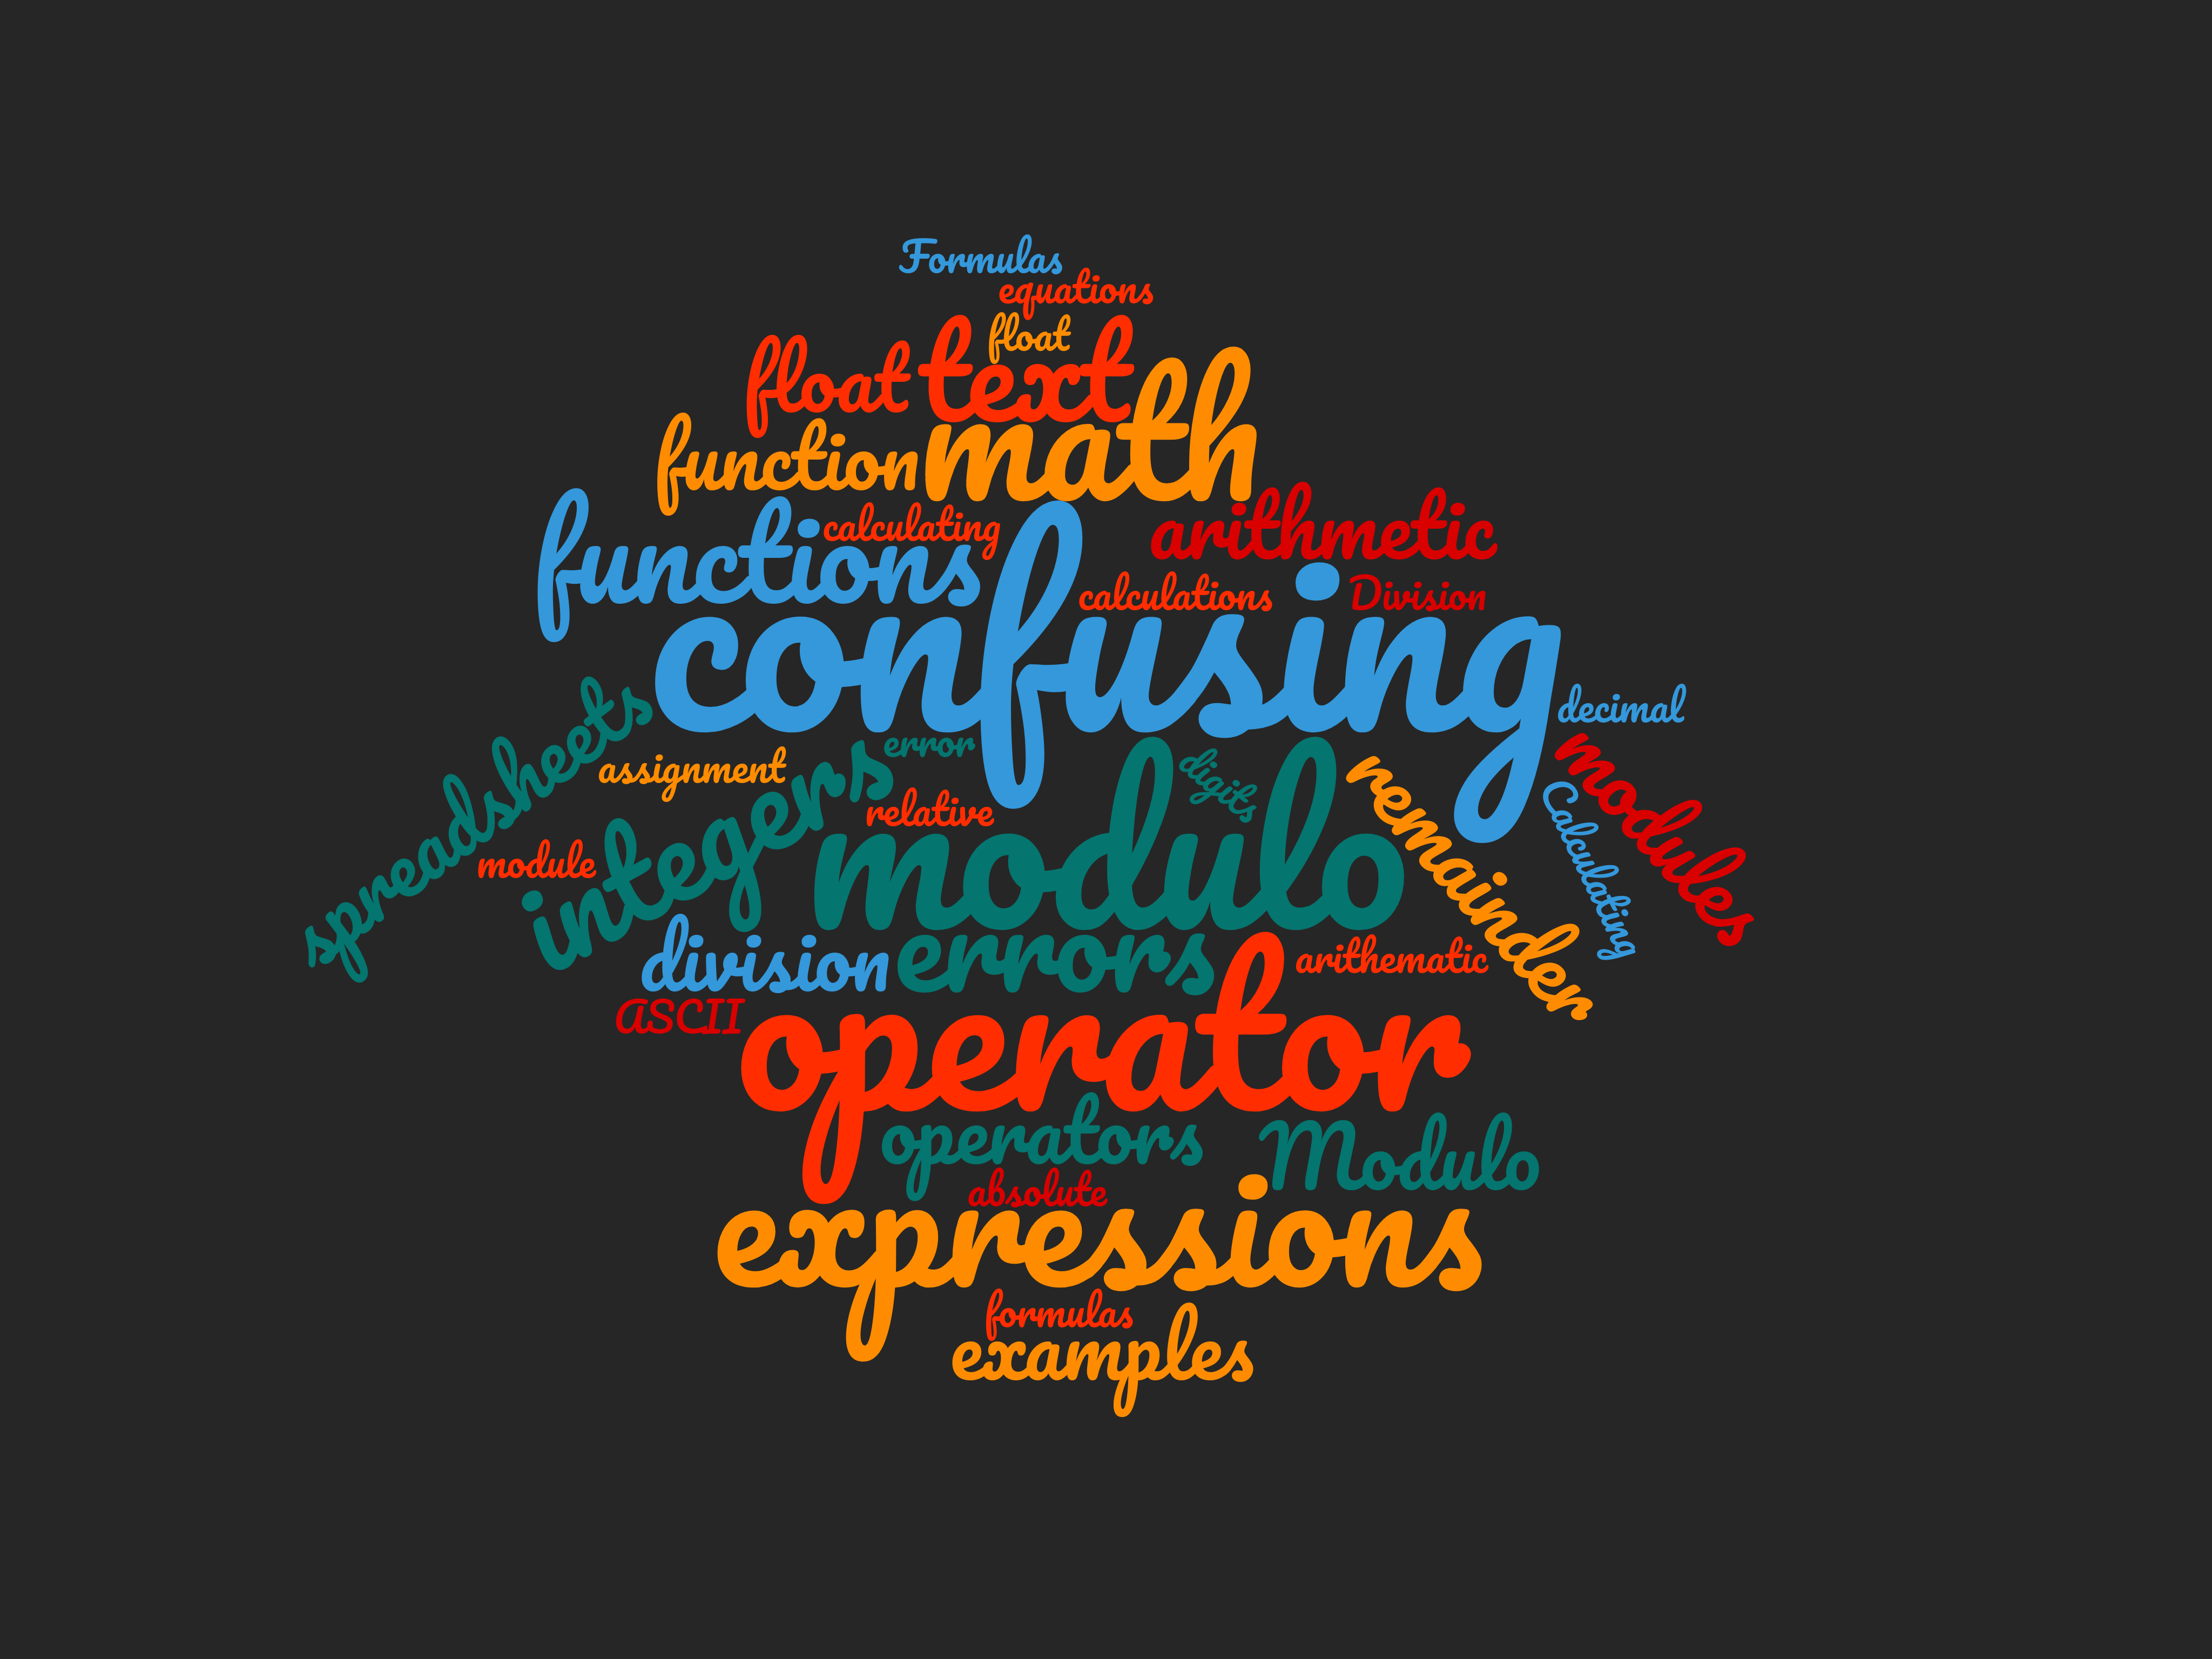
\includegraphics[width=.75\textwidth]{./imgs/muddiest-points-cloud-topic-2.png}
  \end{figure}
\end{frame}

%
%
%
\begin{frame}[fragile]
  \frametitle{Poll Question: Spreadsheets}
  If I copy the contents of B2 to C4 what formula will be in C4?
  \vfill
  \begin{minipage}{.3\textwidth}
    \begin{enumerate}
      \item \lstinline{=$A1 + 2}
      \item \lstinline{=$A2 + 2}
      \item \lstinline{=$A3 + 2}
      \item \lstinline{=$C1 + 2}
      \item \lstinline{=$C2 + 2}
      \item \lstinline{=$C3 + 2}
    \end{enumerate}
  \end{minipage}
  \begin{minipage}{.65\textwidth}
    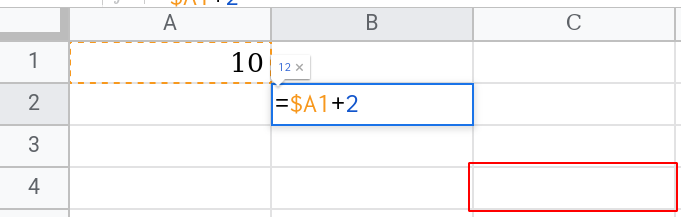
\includegraphics[width=\textwidth]{./imgs/spreadsheet-slide-1.png}
  \end{minipage}
\end{frame}

%
%
%
\begin{frame}[fragile]
  \frametitle{Poll Question: Python Naming}
  Which are legal python names?
  \begin{itemize}
    \item \lstinline{____}
    \item \lstinline{12monkeys}
    \item \lstinline{l33tCoder42}
  \end{itemize}
  \begin{enumerate}
    \item 1 and 2
    \item 1 and 3
    \item 2 only
    \item 2 and 3
    \item 1, 2, and 3
  \end{enumerate}
\end{frame}


%
%
%
\begin{frame}[fragile]
  \frametitle{Poll Question: Program Tracing}
  What is the value of y after this code executes?
  \begin{lstlisting}[language=Python]
  x = 2
  y = x + 3
  x = 5
  \end{lstlisting}
  \begin{enumerate}
    \item 2
    \item 3
    \item 5
    \item 8
    \item 10
  \end{enumerate}
\end{frame}

%
%
%
\begin{frame}[fragile]
  \frametitle{Poll Question: Program Tracing}
  What get outputted to the screen as a result of running the following program if the user types in 5?
  \begin{lstlisting}[language=Python]
  x = input(Enter a number: )
  y = x + 3
  print(y)
  \end{lstlisting}
  \begin{enumerate}
    \item TypeError
    \item SyntaxError
    \item 53
    \item 8
  \end{enumerate}
\end{frame}

%
%
%
\begin{frame}[fragile]
  \frametitle{Poll Question: Program Tracing}
  Result of running this code if the user types in 2 and 10?
  \begin{lstlisting}[language=Python]
  x = int(input())
  y = int(input())
  z = x + y
  print(z)
  \end{lstlisting}
  \begin{enumerate}
    \item TypeError
    \item SyntaxError
    \item 12
    \item 210
  \end{enumerate}
\end{frame}

%
%
%
\begin{frame}[fragile]
  \frametitle{Poll Question: Spreadsheets}
  What will be the expression when the cell at B1 is copied to D4?
  \vfill
  \begin{minipage}{.29\textwidth}
    \begin{enumerate}
      \item \lstinline{=$C$1+$C2}
      \item \lstinline{=$A$1+$D4}
      \item \lstinline{=$A$5+$A2}
      \item \lstinline{=$A$1+$A4}
      \item \lstinline{=$A$1+$A5}
    \end{enumerate}
  \end{minipage}
  \begin{minipage}{.69\textwidth}
    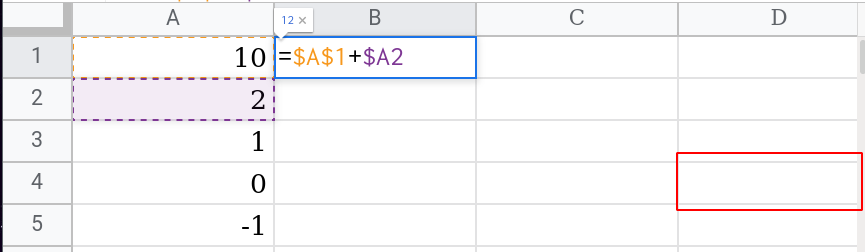
\includegraphics[width=\textwidth]{./imgs/spreadsheet-slide-2.png}
  \end{minipage}
\end{frame}

%
%
%
\begin{frame}[fragile]
  \frametitle{Poll Question: Whitespace}
  Which of the following are considered \'whitespace\'?
  \vfill
  \begin{enumerate}
    \item Spaces
    \item Tabs
    \item Newlines
    \item Spaces and Tabs
    \item Spaces, Tabs, and Newlines
  \end{enumerate}
  \pause
  \vfill
  Whitespace is any character that takes up vertical or horizontal space bu does not produce an otherwise visible mark.
\end{frame}


%
%
%
\section{Topic Review: Escape Character}
\begin{frame}[fragile]
  \frametitle{Topic Review: Escape Character}
  \begin{enumerate}
    \item Treat backslash(\textbackslash) as a special character
    \item \textbackslash means that the character \textit{immediatly} following it should be treated differently.
      \begin{enumerate}
        \item \lstinline{\' and \"} escape quotes within a string.
        \item \lstinline{\t} encodes a tab.
        \item \lstinline{\n} encodes a new line.
        \item \lstinline{\\} encodes a slash.
      \end{enumerate}
  \end{enumerate}
\end{frame}

%
%
%
\begin{frame}[fragile]
  \frametitle{Poll Question: }
  How many of the following characters are visible on the screen?\\
  \begin{lstlisting}[language=Python]
  print('\t\\n\\\t')
  \end{lstlisting}
  \vfill
  \begin{minipage}{.48\textwidth}
    \begin{enumerate}
      \item 1
      \item 2
      \item 3
      \item 4
      \item 5
    \end{enumerate}
  \end{minipage}
  \begin{minipage}{.48\textwidth}
  \end{minipage}
\end{frame}

%
%
%
\begin{frame}[fragile]
  \frametitle{Poll Question: Python Literals}
  Which of the following is not a valid Python literal?
  \begin{enumerate}
    \item 1.00001
    \item 1E-7
    \item 1,097
    \item -3.00
    \item \lstinline{'\'\'''}
  \end{enumerate}
\end{frame}


\section{Topic Review: More Math Operators}

%
%
%
\begin{frame}[fragile]
  \frametitle{Division, Floor Division, and Modulo}
  \begin{enumerate}
    \item Division operator (/) gives best approximation to true result and \textit{always return a float}.
    \item Floor division (//) rounds down the closet whole number. The type of the result will follow the normal rules.
    \item Modulo operator(\%) performs a division and returns the remainder. The type of the result will always be the same.
    \item For any numbers x and y, the following equality holds: \lstinline{(y == (y // x) * x + (y % x))}
  \end{enumerate}
\end{frame}

%
%
%
\begin{frame}[fragile]
  \frametitle{Poll Question: More Math Operators}
  \vfill
  Which computes how many (whole) apples I can give to each friend?
  \begin{enumerate}
    \item \lstinline{num_friends / num_apples}
    \item \lstinline{num_apples / num_friends}
    \item \lstinline{num_friends // num_apples}
    \item \lstinline{num_apples // num_friends}
    \item \lstinline{num_friends % num_appples}
    \item \lstinline{num_apples % num_friends}
  \end{enumerate}
\end{frame}


\section{Topic Review: Orders of Operation}

\begin{frame}
  \frametitle{Order of Operations in Python}
  \centering
  \begin{minipage}{0.49\textwidth}
    \begin{itemize}
      \item Parentheses precedence
      \item Exponentiation
      \item Positive and negative
      \item Multiplication, Division, Modulo
      \item Addition, Subtraction precedence
    \end{itemize}
  \end{minipage}
  \begin{minipage}{0.2\textwidth}
    \centering
    Highest\\
    $\xdownarrow{2cm}$\\
    Lowest\\
  \end{minipage}
  \vfill\\
  \textbf{Note:} Python evaluates from left to right within a precedence level
\end{frame}



%
%
%
\begin{frame}
  \begin{enumerate}
    \item Homework 2 is posted:
      \begin{enumerate}
        \item Due at 11pm (CST) this Friday (June 25)
        \item Covers two topics:
          \begin{enumerate}
            \item Topic 2 - Today's lecture and your last reading
            \item Topic 3 - Wednesday's lecture. 
          \end{enumerate}
        \item \textbf{Start homework early}
      \end{enumerate}
    \item Post-Reading 3 and zyBook topic 3 participation activities due tommorow at 11:00pm (CST).
    \item \textbf{First quiz this Thursday so please sign-up at the CBTF's scheduler.}
      \begin{enumerate}
        \item http://cbtf.engr.illinois.edu/sched/
        \item includes interface for requesting conflict exams
      \end{enumerate}
  \end{enumerate}
\end{frame}

\end{document}
